\documentclass[12pt]{article}

% Computational Physics by M. Newman
% Setup file for exercises

% Packages
\usepackage{mathpazo}
\usepackage{amsmath}
\usepackage{graphicx}
\usepackage{calrsfs}
\usepackage{fancyvrb}

% Formatting
\setlength{\textwidth}{17.5cm}
\setlength{\textheight}{24.0cm}
\setlength{\evensidemargin}{2.5cm}
\setlength{\oddsidemargin}{-0.6cm}
\setlength{\topmargin}{-2.3cm}
\setlength{\textfloatsep}{0pt}
\setcounter{secnumdepth}{0}
\renewcommand{\baselinestretch}{1.06}

% Macros
\newcommand{\dd}{\mathrm{d}}
\newcommand{\ii}{\mathrm{i}}
\newcommand{\e}{\mathrm{e}}
\newcommand{\half}{\tfrac12}
\newcommand{\av}[1]{\langle#1\rangle}
\newcommand{\var}{\mathop\mathrm{var}}
\newcommand{\Ord}{\mathrm{O}}
\renewcommand{\Re}{\mathop\mathrm{Re}\nolimits}
\renewcommand{\Im}{\mathop\mathrm{Im}\nolimits}
\newcommand{\mat}{\mathbf}
\renewcommand{\vec}{\mathbf}
\newcommand{\defn}{\textit}
\newcommand{\exskip}{\nopagebreak\medskip\noindent}
\newcommand{\pmstrut}{\rule{0pt}{13pt}}

% Environments
\newcounter{chapter}
\setcounter{chapter}{2}
\newcounter{exercise}
\renewcommand{\theexercise}{\arabic{chapter}.\arabic{exercise}}
\newenvironment{exercises}{\vspace{2ex plus0.5ex minus0.5ex}
  \renewcommand{\labelenumi}{\alph{enumi})}}%
    {\par\vspace{1ex plus0.5ex minus0.5ex}}
\newcommand{\exercise}{\refstepcounter{exercise}%
  \par\vspace{4ex plus1ex minus1ex}%
  \noindent\textbf{Exercise \theexercise: }}

\DefineVerbatimEnvironment{code}{Verbatim}{xleftmargin=\parindent}

\setcounter{chapter}{8}

\begin{document}

\noindent {\LARGE\textsc{Computational Physics}}\par
\bigskip
\noindent {\large\textsc{Exercises for Chapter \arabic{chapter}}}\par
\noindent\hrulefill

%%%%%%%%%%%%%%%%%%%%%%%%%%%%%%%%%%%%%%%%%%%%%%%%%%%%%%%%%%%%%%%%%%%%%%
%%%                                                                %%%
%%%     COMPUTATIONAL PHYSICS, M. NEWMAN, CHAPTER 8, EXERCISES     %%%
%%%                                                                %%%
%%%%%%%%%%%%%%%%%%%%%%%%%%%%%%%%%%%%%%%%%%%%%%%%%%%%%%%%%%%%%%%%%%%%%%

\begin{exercises}

%%% Exercise 8.1 %%%

\exercise \textbf{A low-pass filter}

\exskip Here is a simple electronic circuit
with one resistor and one capacitor:
\smallskip
\begin{center}
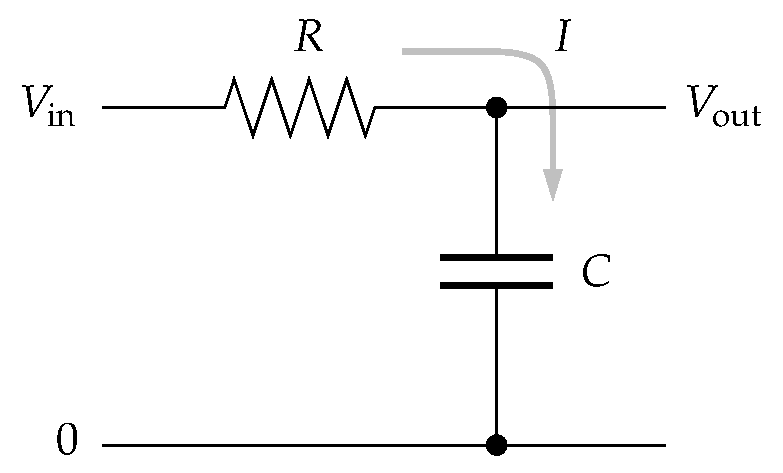
\includegraphics[width=7cm]{lowpass.eps}
\end{center}
\smallskip
This circuit acts as a low-pass filter: you send a signal in on the left
and it comes out filtered on the right.

Using Ohm's law and the capacitor law and assuming that the output load has
very high impedance, so that a negligible amount of current flows through
it, we can write down the equations governing this circuit as follows.  Let
$I$ be the current that flows through~$R$ and into the capacitor, and let
$Q$ be the charge on the capacitor.  Then:
\begin{displaymath}
IR = V_\textrm{in} - V_\textrm{out}\,,\qquad
 Q = CV_\textrm{out}\,,\qquad
 I = {\dd Q\over\dd t}.
\end{displaymath}
Substituting the second equation into the third, then substituting the
result into the first equation, we find that $V_\textrm{in} -
V_\textrm{out} = RC\>({\dd V_\textrm{out}/\dd t})$, or equivalently
\begin{displaymath}
{\dd V_\textrm{out}\over\dd t} = {1\over RC}
                               \bigl( V_\textrm{in} - V_\textrm{out} \bigr).
\end{displaymath}

\begin{enumerate}\setlength{\itemsep}{0pt}
\item Write a program (or modify a previous one) to solve this equation for
  $V_\textrm{out}(t)$ using the fourth-order Runge--Kutta method when in
  the input signal is a square-wave with frequency~1 and amplitude~1:
\begin{equation}
V_\textrm{in}(t) = \begin{cases}
                     1  & \qquad\mbox{if $\lfloor 2t \rfloor$ is even,} \\
                     -1 & \qquad\mbox{if $\lfloor 2t \rfloor$ is odd,}
                   \end{cases}
\end{equation}
where $\lfloor x\rfloor$ means $x$ rounded down to the next lowest integer.
Use the program to make plots of the output of the filter circuit from
$t=0$ to $t=10$ when $RC=0.01$, $0.1$, and~1, with initial
condition~$V_\textrm{out}(0)=0$.  You will have to make a decision about
what value of $h$ to use in your calculation.  Small values give more
accurate results, but the program will take longer to run.  Try a variety
of different values and choose one for your final calculations that seems
sensible to you.
\item Based on the graphs produced by your program, describe what you see
  and explain what the circuit is doing.
\end{enumerate}

A program similar to the one you wrote is running inside most stereos and
music players, to create the effect of the ``bass'' control.  In the old
days, the bass control on a stereo would have been connected to a real
electronic low-pass filter in the amplifier circuitry, but these days there
is just a computer processor that simulates the behavior of the filter in a
manner similar to your program.


%%% Exercise 8.2 %%%

\exercise \textbf{The Lotka--Volterra equations}

\exskip The Lotka--Volterra equations are a
mathematical model of predator--prey interactions between biological
species.  Let two variables $x$ and $y$ be proportional to the size of the
populations of two species, traditionally called ``rabbits'' (the
prey) and ``foxes'' (the predators).  You could think of $x$ and $y$ as
being the population in thousands, say, so that $x=2$ means there are 2000
rabbits.  Strictly the only allowed values of $x$ and~$y$ would then be
multiples of 0.001, since you can only have whole numbers of rabbits or
foxes.  But 0.001 is a pretty close spacing of values, so it's a decent
approximation to treat $x$ and $y$ as continuous real numbers so long as
neither gets very close to zero.

In the Lotka--Volterra model the rabbits reproduce at a rate proportional
to their population, but are eaten by the foxes at a rate proportional to
both their own population and the population of foxes:
\begin{displaymath}
{\dd x\over\dd t} = \alpha x - \beta xy,
\end{displaymath}
where $\alpha$ and $\beta$ are constants.  At the same time the foxes
reproduce at a rate proportional the rate at which they eat
rabbits---because they need food to grow and reproduce---but also die of
old age at a rate proportional to their own population:
\begin{displaymath}
{\dd y\over\dd t} = \gamma xy - \delta y,
\end{displaymath}
where $\gamma$ and $\delta$ are also constants.

\begin{enumerate}\setlength{\itemsep}{0pt}
\item Write a program to solve these equations using the fourth-order
  Runge--Kutta method for the case $\alpha=1$, $\beta=\gamma=0.5$, and
  $\delta=2$, starting from the initial condition $x=y=2$.  Have the
  program make a graph showing both $x$ and $y$ as a function of time on
  the same axes from $t=0$ to $t=30$.  (Hint: Notice that the differential
  equations in this case do not depend explicitly on time~$t$---in vector
  notation, the right-hand side of each equation is a function $f(\vec{r})$
  with no $t$ dependence.  You may nonetheless find it convenient to define
  a Python function \verb|f(r,t)| including the time variable, so that your
  program takes the same form as programs given earlier in this chapter.
  You don't have to do it that way, but it can avoid some confusion.
  Several of the following exercises have a similar lack of explicit
  time-dependence.)
\item Describe in words what is going on in the system, in terms of rabbits
  and foxes.
\end{enumerate}


%%% Exercise 8.3 %%%

\exercise \textbf{The Lorenz equations}

\exskip One of the most celebrated sets of differential equations in
physics is the Lorenz equations:
\begin{displaymath}
{\dd x\over\dd t} = \sigma(y-x),\qquad
{\dd y\over\dd t} = rx - y - xz,\qquad
{\dd z\over\dd t} = xy - bz,
\end{displaymath}
where $\sigma$, $r$, and~$b$ are constants.  (The names $\sigma$, $r$,
and~$b$ are odd, but traditional---they are always used in these equations
for historical reasons.)

These equations were first studied by Edward Lorenz in 1963, who
derived them from a simplified model of weather patterns.  The
reason for their fame is that they were one of the first incontrovertible
examples of \defn{deterministic chaos}, the occurrence of apparently
random motion even though there is no randomness built into the equations.
We encountered a different example of chaos in the logistic map of
Exercise~3.6.
\begin{enumerate}\setlength{\itemsep}{0pt}
\item Write a program to solve the Lorenz equations for the case
  $\sigma=10$, $r=28$, and~$b=\frac83$ in the range from $t=0$ to $t=50$
  with initial conditions $(x,y,z)=(0,1,0)$.  Have your program make a plot
  of $y$ as a function of time.  Note the unpredictable nature of the
  motion.  (Hint: If you base your program on previous ones, be careful.
  This problem has parameters $r$ and $b$ with the same names as variables
  in previous programs---make sure to give your variables new names, or use
  different names for the parameters, to avoid introducing errors into your
  code.)
\item Modify your program to produce a plot of $z$ against~$x$.  You should
  see a picture of the famous ``strange attractor'' of the Lorenz
  equations, a lop-sided butterfly-shaped plot that never repeats itself.
\end{enumerate}


%%% Exercise 8.4 %%%

\exercise Building on the results from Example~8.6 above, calculate the
motion of a nonlinear pendulum as follows.
\begin{enumerate}\setlength{\itemsep}{0pt}
\item Write a program to solve the two first-order equations, Eqs.~(8.45)
  and~(8.46), using the fourth-order Runge--Kutta method for a pendulum
  with a $10\,$cm arm.  Use your program to calculate the angle~$\theta$ of
  displacement for several periods of the pendulum when it is released from
  a standstill at $\theta=179^\circ$ from the vertical.  Make a graph
  of~$\theta$ as a function of time.
\item Extend your program to create an animation of the motion of the
  pendulum.  Your animation should, at a minimum, include a representation
  of the moving pendulum bob and the pendulum arm.  (Hint: You will
  probably find the function \verb|rate| discussed in Section~3.5 useful
  for making your animation run at a sensible speed.  Also, you may want to
  make the step size for your Runge--Kutta calculation smaller than the
  frame-rate of your animation, i.e.,~do several Runge--Kutta steps per
  frame on screen.  This is certainly allowed and may help to make your
  calculation more accurate.)
\end{enumerate}
For a bigger challenge, take a look at Exercise~8.15 on page~398, which
invites you to write a program to calculate the chaotic motion of the
double pendulum.


%%% Exercise 8.5 %%%

\exercise \textbf{The driven pendulum}

\exskip A pendulum like the one in Exercise~8.4 can be driven by, for
example, exerting a small oscillating force horizontally on the mass.  Then
the equation of motion for the pendulum becomes
\begin{displaymath}
{\dd^2\theta\over\dd t^2} = - {g\over\ell}\sin\theta
  + C \cos\theta \sin\Omega t,
\end{displaymath}
where $C$ and $\Omega$ are constants.
\begin{enumerate}\setlength{\itemsep}{0pt}
\item Write a program to solve this equation for $\theta$ as a function of
  time with $\ell=10\,$cm, $C=2\,\mathrm{s}^{-2}$ and
  $\Omega=5\,\mathrm{s}^{-1}$ and make a plot of $\theta$ as a function of
  time from $t=0$ to $t=100\,$s.  Start the pendulum at rest with
  $\theta=0$ and $\dd\theta/\dd t=0$.
\item Now change the value of~$\Omega$, while keeping~$C$ the same, to find
  a value for which the pendulum resonates with the driving force and
  swings widely from side to side.  Make a plot for this case also.
\end{enumerate}


%%% Exercise 8.6 %%%

\exercise \textbf{Harmonic and anharmonic oscillators}

\exskip The simple harmonic oscillator arises in many physical problems, in
mechanics, electricity and magnetism, and condensed matter physics, among
other areas.  Consider the standard oscillator equation
\begin{displaymath}
{\dd^2 x\over\dd t^2} = -\omega^2 x.
\end{displaymath}
\begin{enumerate}\setlength{\itemsep}{0pt}
\item Using the methods described in the preceding section, turn this
  second-order equation into two coupled first-order equations.  Then write
  a program to solve them for the case $\omega=1$ in the range from $t=0$
  to $t=50$.  A second-order equation requires two initial conditions, one
  on $x$ and one on its derivative.  For this problem use $x=1$ and $\dd
  x/\dd t = 0$ as initial conditions.  Have your program make a graph
  showing the value of $x$ as a function of time.
\item Now increase the amplitude of the oscillations by making the initial
  value of $x$ bigger---say $x=2$---and confirm that the period of the
  oscillations stays roughly the same.
\item Modify your program to solve for the motion of the anharmonic
  oscillator described by the equation
\begin{displaymath}
{\dd^2 x\over\dd t^2} = -\omega^2 x^3.
\end{displaymath}
Again take $\omega=1$ and initial conditions $x=1$ and $\dd x/\dd t=0$ and
make a plot of the motion of the oscillator.  Again increase the amplitude.
You should observe that the oscillator oscillates faster at higher
amplitudes.  (You can try lower amplitudes too if you like, which should be
slower.)  The variation of frequency with amplitude in an anharmonic
oscillator was studied previously in Exercise~5.10.
\item Modify your program so that instead of plotting $x$ against~$t$, it
  plots $\dd x/\dd t$ against $x$, i.e.,~the ``velocity'' of the oscillator
  against its ``position.''  Such a plot is called a \defn{phase
    space} plot.
\item The \defn{van der Pol oscillator}, which appears in electronic
  circuits and in laser physics, is described by the equation
\begin{displaymath}
{\dd^2 x\over\dd t^2} - \mu (1-x^2) {\dd x\over\dd t} + \omega^2 x = 0.
\end{displaymath}
Modify your program to solve this equation from $t=0$ to $t=20$ and hence
make a phase space plot for the van der Pol oscillator with $\omega=1$,
$\mu=1$, and initial conditions $x=1$ and $\dd x/\dd t=0$.  Try it also for
$\mu=2$ and $\mu=4$ (still with $\omega=1$).  Make sure you use a small
enough value of the time interval~$h$ to get a smooth, accurate phase space
plot.
\end{enumerate}


%%% Exercise 8.7 %%%

\exercise \textbf{Trajectory with air resistance}

\exskip Many elementary mechanics problems deal with the physics of objects
moving or flying through the air, but they almost always ignore friction
and air resistance to make the equations solvable.  If we're using a
computer, however, we don't need solvable equations.

Consider, for instance, a spherical cannonball shot from a cannon standing
on level ground.  The air resistance on a moving sphere is a force in the
opposite direction to the motion with magnitude
\begin{displaymath}
F = \half \pi R^2\rho C v^2,
\end{displaymath}
where $R$ is the sphere's radius, $\rho$~is the density of air, $v$~is the
velocity, and $C$~is the so-called \defn{coefficient of drag} (a
property of the shape of the moving object, in this case a sphere).
\begin{enumerate}\setlength{\itemsep}{0pt}
\item Starting from Newton's second law, $F=ma$, show that the
  equations of motion for the position $(x,y)$ of the cannonball are
\begin{displaymath}
\ddot{x} = - {\pi R^2\rho C\over2m}\,
             \dot{x}\sqrt{\dot{x}^2+\dot{y}^2},
\qquad
\ddot{y} =  - g - {\pi R^2\rho C\over2m}\,
             \dot{y}\sqrt{\dot{x}^2+\dot{y}^2},
\end{displaymath}
where $m$ is the mass of the cannonball, $g$ is the acceleration due to
gravity, and $\dot{x}$ and $\ddot{x}$ are the first and second derivatives
of~$x$ with respect to time.
\item Change these two second-order equations into four first-order
  equations using the methods you have learned, then write a program that
  solves the equations for a cannonball of mass $1\,$kg and radius $8\,$cm,
  shot at $30^\circ$ to the horizontal with initial velocity
  $100\,\mathrm{ms}^{-1}$.  The density of air is
  $\rho=1.22\,\textrm{kg}\,\textrm{m}^{-3}$ and the coefficient of drag for
  a sphere is $C=0.47$.  Make a plot of the trajectory of the cannonball
  (i.e.,~a graph of $y$ as a function of~$x$).
\item When one ignores air resistance, the distance traveled by a
  projectile does not depend on the mass of the projectile.  In real life,
  however, mass certainly does make a difference.  Use your program to
  estimate the total distance traveled (over horizontal ground) by the
  cannonball above, and then experiment with the program to determine
  whether the cannonball travels further if it is heavier or lighter.  You
  could, for instance, plot a series of trajectories for cannonballs of
  different masses, or you could make a graph of distance traveled as a
  function of mass.  Describe briefly what you discover.
\end{enumerate}


%%% Exercise 8.8 %%%

\exercise \textbf{Space garbage}

\exskip A heavy steel rod and a spherical
ball-bearing, discarded by a passing spaceship, are floating in zero
gravity and the ball bearing is orbiting around the rod under the effect of
its gravitational pull:
\begin{center}
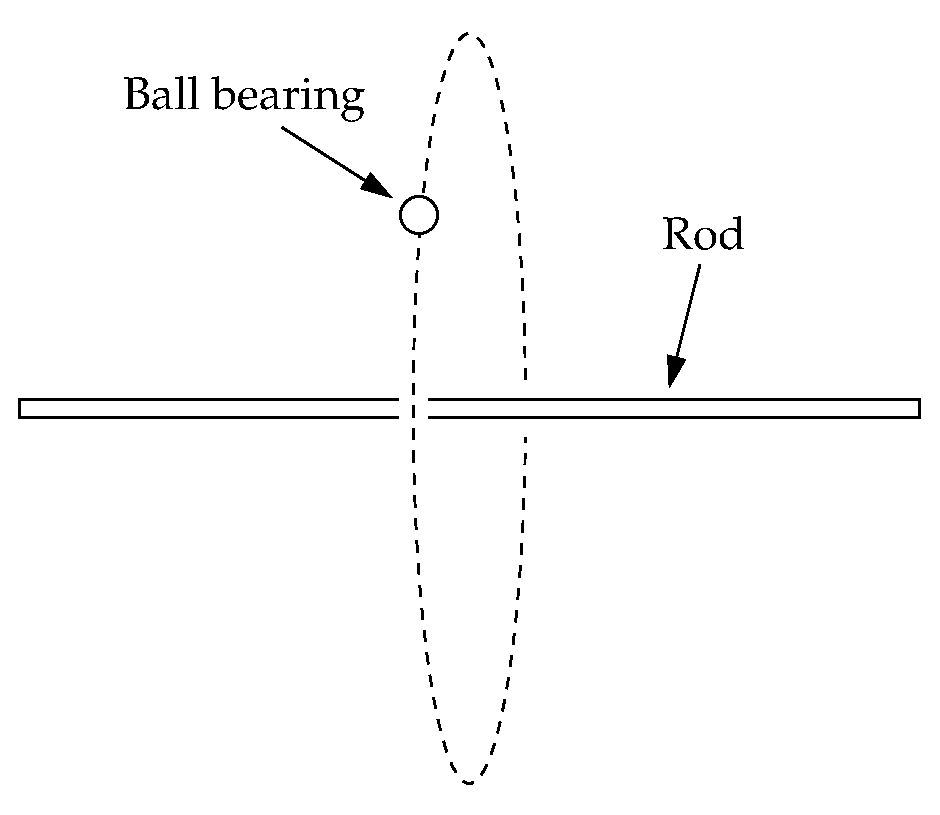
\includegraphics[width=7.5cm]{rod.eps}
\end{center}
For simplicity we'll assume that the rod is of negligible cross-section and
heavy enough that it doesn't move significantly, and that the ball bearing
is orbiting around the rod's mid-point in a plane perpendicular to the rod.
\begin{enumerate}\setlength{\itemsep}{0pt}
\item Treating the rod as a line of mass~$M$ and length~$L$ and the ball
  bearing as a point mass~$m$, show that the attractive force~$F$ felt by
  the ball bearing in the direction toward the center of the rod is given
  by
\begin{displaymath}
F = {GMm\over L} \sqrt{x^2+y^2}
    \int_{-L/2}^{L/2} {\dd z\over(x^2+y^2+z^2)^{3/2}}\,,
\end{displaymath}
where $G$ is Newton's gravitational constant and $x$ and $y$ are the
coordinates of the ball bearing in the plane perpendicular to the rod.  The
integral can be done in closed form and gives
\begin{displaymath}
F = {GMm\over\sqrt{(x^2+y^2)(x^2+y^2+L^2/4)}}.
\end{displaymath}
Hence show that the equations of motion for the position $x,y$ of the ball
bearing in the $xy$-plane are
\begin{displaymath}
{\dd^2 x\over\dd t^2} = - GM {x\over r^2\sqrt{r^2+L^2/4}},\qquad
{\dd^2 y\over\dd t^2} = - GM {y\over r^2\sqrt{r^2+L^2/4}},
\end{displaymath}
where $r=\sqrt{x^2+y^2}$.
\item Convert these two second-order equations into four first-order ones
  using the techniques of Section~8.3.  Then, working in units where~$G=1$,
  write a program to solve them for $M=10$, $L=2$, and initial conditions
  $(x,y)=(1,0)$ with velocity of $+1$ in the $y$ direction.  Calculate the
  orbit from $t=0$ to $t=10$ and make a plot of it, meaning a plot of $y$
  against~$x$.  You should find that the ball bearing does not orbit in a
  circle or ellipse as a planet does, but has a precessing orbit, which
  arises because the attractive force is not a simple $1/r^2$ force as it
  is for a planet orbiting the Sun.
\end{enumerate}


%%% Exercise 8.9 %%%

\exercise \textbf{Vibration in a one-dimensional system}

\exskip In Example~6.2 on page~235 we studied the motion of a system of $N$
identical masses (in zero gravity) joined by identical linear springs like
this: \medskip
\begin{center}
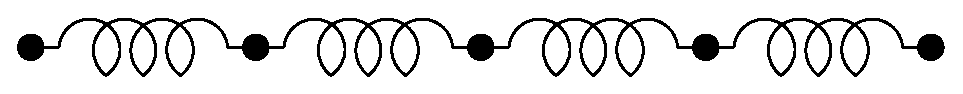
\includegraphics[width=9cm]{springs.eps}
\end{center}
As we showed, the horizontal displacements~$\xi_i$ of masses~$i=1\ldots N$
satisfy equations of motion
\begin{align*}
m {\dd^2\xi_1\over\dd t^2} &= k(\xi_2-\xi_1) + F_1,\\
m {\dd^2\xi_i\over\dd t^2} &= k(\xi_{i+1}-\xi_i) + k(\xi_{i-1}-\xi_i) + F_i\,,
  \\
m {\dd^2\xi_N\over\dd t^2} &= k(\xi_{N-1}-\xi_N) + F_N.
\end{align*}
where $m$ is the mass, $k$ is the spring constant, and $F_i$ is the
external force on mass~$i$.  In Example~6.2 we showed how these equations
could be solved by guessing a form for the solution and using a matrix
method.  Here we'll solve them more directly.
\begin{enumerate}\setlength{\itemsep}{0pt}
\item Write a program to solve for the motion of the masses using the
  fourth-order Runge--Kutta method for the case we studied previously where
  $m=1$ and $k=6$, and the driving forces are all zero except for $F_1 =
  \cos\omega t$ with $\omega=2$.  Plot your solutions for the
  displacements~$\xi_i$ of all the masses as a function of time from $t=0$
  to $t=20$ on the same plot.  Write your program to work with
  general~$N$, but test it out for small values---$N=5$ is a reasonable
  choice.

  You will need first of all to convert the $N$ second-order equations of
  motion into~$2N$ first-order equations.  Then combine all of the
  dependent variables in those equations into a single large
  vector~$\vec{r}$ to which you can apply the Runge--Kutta method in the
  standard fashion.
\item Modify your program to create an animation of the movement of the
  masses, represented as spheres on the computer screen.  You will probably
  find the \verb|rate| function discussed in Section~3.5 useful for making
  your animation run at a sensible speed.
\end{enumerate}


%%% Exercise 8.10 %%%

\exercise \textbf{Cometary orbits}

\exskip Many comets travel in highly elongated orbits around the Sun.  For
much of their lives they are far out in the solar system, moving very
slowly, but on rare occasions their orbit brings them close to the Sun for
a fly-by and for a brief period of time they move very fast indeed:
\bigskip
\begin{center}
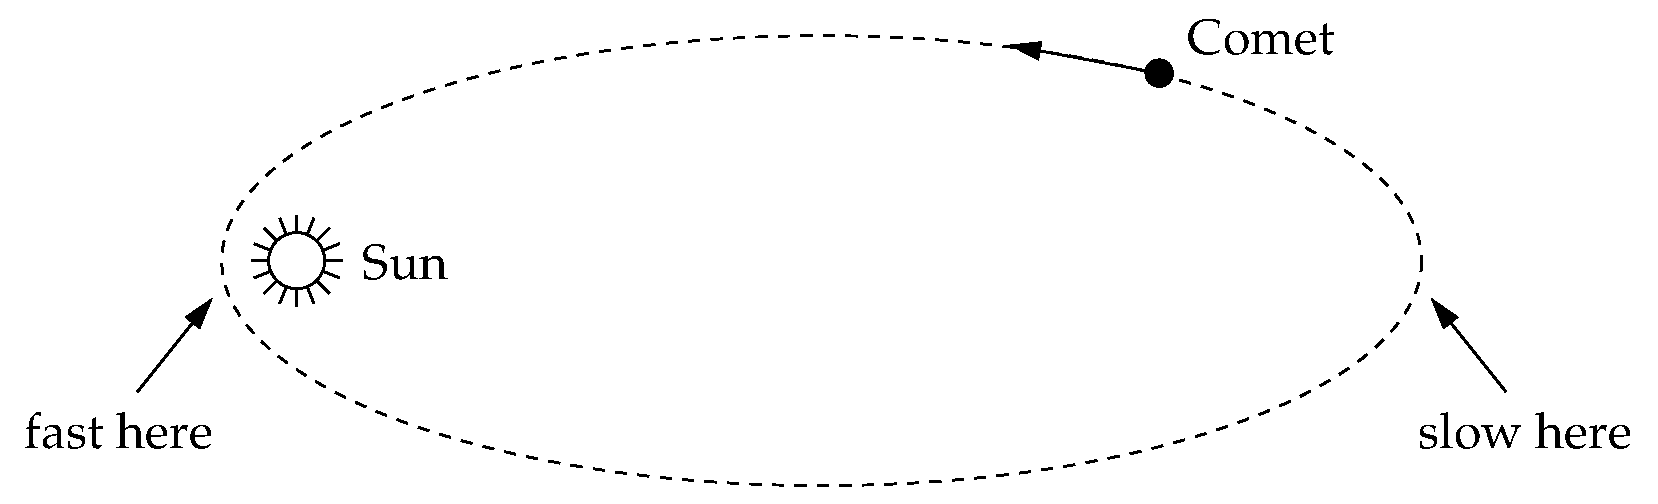
\includegraphics[width=12cm]{orbit.eps}
\end{center}
\bigskip This is a classic example of a system for which an adaptive
step size method is useful, because for the large periods of time when the
comet is moving slowly we can use long time-steps, so that the program runs
quickly, but short time-steps are crucial in the brief but fast-moving
period close to the Sun.

The differential equation obeyed by a comet is straightforward to
derive.  The force between the Sun, with mass~$M$ at the origin, and a
comet of mass~$m$ with position vector~$\vec{r}$ is $GMm/r^2$ in direction
$-\vec{r}/r$ (i.e.,~the direction towards the Sun), and hence Newton's
second law tells us that
\begin{displaymath}
m {\dd^2\vec{r}\over\dd t^2} = -\biggl({GMm\over r^2}\biggr)\,{\vec{r}\over r}.
\end{displaymath}
Canceling the~$m$ and taking the $x$ component we have
\begin{displaymath}
{\dd^2 x\over\dd t^2} = -GM {x\over r^3}\,,
\end{displaymath}
and similarly for the other two coordinates.  We can, however, throw out
one of the coordinates because the comet stays in a single plane as it
orbits.  If we orient our axes so that this plane is perpendicular to
the~$z$-axis, we can forget about the $z$ coordinate and we are left with
just two second-order equations to solve:
\begin{displaymath}
{\dd^2 x\over\dd t^2} = -GM {x\over r^3}\,, \qquad
{\dd^2 y\over\dd t^2} = -GM {y\over r^3}\,,
\end{displaymath}
where $r=\sqrt{x^2+y^2}$.

\begin{enumerate}\setlength{\itemsep}{0pt}
\item Turn these two second-order equations into four first-order
  equations, using the methods you have learned.
\item Write a program to solve your equations using the fourth-order
  Runge--Kutta method with a \emph{fixed} step size.  You will need to look
  up the mass of the Sun and Newton's gravitational constant~$G$.  As an
  initial condition, take a comet at coordinates $x=4$~billion kilometers
  and $y=0$ (which is somewhere out around the orbit of Neptune) with
  initial velocity $v_x=0$ and $v_y = 500\,\mathrm{m\,s}^{-1}$.  Make a
  graph showing the trajectory of the comet (i.e.,~a plot of $y$
  against~$x$).

  Choose a fixed step size~$h$ that allows you to accurately calculate at
  least two full orbits of the comet.  Since orbits are periodic, a good
  indicator of an accurate calculation is that successive orbits of the
  comet lie on top of one another on your plot.  If they do not then you
  need a smaller value of~$h$.  Give a short description of your findings.
  What value of $h$ did you use?  What did you observe in your simulation?
  How long did the calculation take?
\item Make a copy of your program and modify the copy to do the calculation
  using an adaptive step size.  Set a target accuracy of
  $\delta=1$~kilometer per year in the position of the comet and again plot
  the trajectory.  What do you see?  How do the speed, accuracy, and step
  size of the calculation compare with those in part~(b)?
\item Modify your program to place dots on your graph showing the position
  of the comet at each Runge--Kutta step around a single orbit.  You should
  see the steps getting closer together when the comet is close to the Sun
  and further apart when it is far out in the solar system.
\end{enumerate}

Calculations like this can be extended to cases where we have more than one
orbiting body---see Exercise~8.16 for an example.  We can include planets,
moons, asteroids, and others.  Analytic calculations are impossible for
such complex systems, but with careful numerical solution of differential
equations we can calculate the motions of objects throughout the entire
solar system.


%%% Exercise 8.11 %%%

\exercise Write a program to solve the differential equation
\begin{displaymath}
{\dd^2 x\over\dd t^2} - \biggl( {\dd x\over\dd t} \biggr)^2 + x + 5 = 0
\end{displaymath}
using the leapfrog method.  Solve from $t=0$ to $t=50$ in steps of
$h=0.001$ with initial condition $x=1$ and $\dd x/\dd t = 0$.  Make a plot
of your solution showing $x$ as a function of~$t$.


%%% Exercise 8.12 %%%

\exercise \textbf{Orbit of the Earth}

\exskip Use the Verlet method to calculate the orbit of the Earth around
the Sun.  The equations of motion for the position $\vec{r} = (x,y)$ of the
planet in its orbital plane are the same as those for any orbiting body and
are derived in Exercise~8.10 on page~361.  In vector form, they are
\begin{displaymath}
{\dd^2\vec{r}\over\dd t^2} = -GM {\vec{r}\over r^3}\,,
\end{displaymath}
where $G=6.6738\times10^{-11}\,\mathrm{m^3\,kg^{-1}\,s^{-2}}$ is Newton's
gravitational constant and $M=1.9891\times10^{30}\,$kg is the mass of the
Sun.

The orbit of the Earth is not perfectly circular, the planet being
sometimes closer to and sometimes further from the Sun.  When it is at its
closest point, or \defn{perihelion}, it is moving precisely tangentially
(i.e.,~perpendicular to the line between itself and the Sun) and it has
distance $1.4710\times10^{11}\,$m from the Sun and linear velocity
$3.0287\times10^4\,\mathrm{m\,s^{-1}}$.
\begin{enumerate}\setlength{\itemsep}{0pt}
\item Write a program to calculate the orbit of the Earth using the Verlet
  method, Eqs.~(8.77) and~(8.78), with a time-step of $h=1$ hour.  Make a
  plot of the orbit, showing several complete revolutions about the Sun.
  The orbit should be very slightly, but visibly, non-circular.
\item The gravitational potential energy of the Earth is $-GMm/r$, where
  $m=5.9722\times10^{24}\,$kg is the mass of the planet, and its kinetic
  energy is $\half mv^2$ as usual.  Modify your program to calculate both
  of these quantities at each step, along with their sum (which is the
  total energy), and make a plot showing all three as a function of time on
  the same axes.  You should find that the potential and kinetic energies
  vary visibly during the course of an orbit, but the total energy remains
  constant.
\item Now plot the total energy alone without the others and you should be
  able to see a slight variation over the course of an orbit.  Because
  you're using the Verlet method, however, which conserves energy in the
  long term, the energy should always return to its starting value at the
  end of each complete orbit.
\end{enumerate}


%%% Exercise 8.13 %%%

\exercise \textbf{Planetary orbits}

\exskip This exercise asks you to calculate the orbits of two of the
planets using the Bulirsch--Stoer method.  The method gives results
significantly more accurate than the Verlet method used to calculate the
Earth's orbit in Exercise~8.12.

The equations of motion for the position $x,y$ of a planet in its orbital
plane are the same as those for any orbiting body and are derived in
Exercise~8.10 on page~361:
\begin{displaymath}
{\dd^2 x\over\dd t^2} = -GM {x\over r^3}\,, \qquad
{\dd^2 y\over\dd t^2} = -GM {y\over r^3}\,,
\end{displaymath}
where $G=6.6738\times10^{-11}\,\mathrm{m^3\,kg^{-1}\,s^{-2}}$ is Newton's
gravitational constant, $M=1.9891\times10^{30}\,$kg is the mass of the Sun,
and $r=\sqrt{x^2+y^2}$.

Let us first solve these equations for the orbit of the Earth, duplicating
the results of Exercise~8.12, though with greater accuracy.  The Earth's
orbit is not perfectly circular, but rather slightly elliptical.  When it
is at its closest approach to the Sun, its perihelion, it is moving
precisely tangentially (i.e.,~perpendicular to the line between itself and
the Sun) and it has distance $1.4710\times10^{11}\,$m from the Sun and
linear velocity $3.0287\times10^4\,\mathrm{ms^{-1}}$.
\begin{enumerate}\setlength{\itemsep}{0pt}
\item Write a program, or modify the one from Example~8.7, to calculate the
  orbit of the Earth using the Bulirsch--Stoer method to a positional
  accuracy of $1\,$km per year.  Divide the orbit into intervals of length
  $H = 1$~week and then calculate the solution for each interval using the
  combined modified midpoint/Richardson extrapolation method described in
  this section.  Make a plot of the orbit, showing at least one complete
  revolution about the Sun.
\item Modify your program to calculate the orbit of the dwarf planet Pluto.
  The distance between the Sun and Pluto at perihelion is
  $4.4368\times10^{12}\,$m and the linear velocity is
  $6.1218\times10^3\,\mathrm{ms^{-1}}$.  Choose a suitable value for $H$ to
  make your calculation run in reasonable time, while once again giving a
  solution accurate to $1\,$km per year.

  You should find that the orbit of Pluto is significantly
  elliptical---much more so than the orbit of the Earth.  Pluto is a Kuiper
  belt object, similar to a comet, and (unlike true planets) it's typical
  for such objects to have quite elliptical orbits.
\end{enumerate}


%%% Exercise 8.14 %%%

\exercise \textbf{Quantum oscillators}

\exskip Consider the one-dimensional,
time-independent Schr\"odinger equation in a harmonic (i.e., quadratic)
potential $V(x)=V_0 x^2/a^2$, where $V_0$ and~$a$ are constants.
\begin{enumerate}\setlength{\itemsep}{0pt}
\item Write down the Schr\"odinger equation for this problem and convert it
  from a second-order equation to two first-order ones, as in Example~8.9.
  Write a program, or modify the one from Example~8.9, to find the energies
  of the ground state and the first two excited states for these equations
  when $m$ is the electron mass, $V_0=50\,$eV, and $a=10^{-11}\,$m.  Note
  that in theory the wavefunction goes all the way out to $x=\pm\infty$,
  but you can get good answers by using a large but finite interval.  Try
  using $x=-10a$ to $+10a$, with the wavefunction~$\psi=0$ at both
  boundaries.  (In effect, you are putting the harmonic oscillator in a box
  with impenetrable walls.)  The wavefunction is real everywhere, so you
  don't need to use complex variables, and you can use evenly spaced points
  for the solution---there is no need to use an adaptive method for this
  problem.

  The quantum harmonic oscillator is known to have energy states that are
  equally spaced.  Check that this is true, to the precision of your
  calculation, for your answers.  (Hint: The ground state has energy in the
  range 100 to $200\,$eV.)
\item Now modify your program to calculate the same three energies for the
  anharmonic oscillator with $V(x) = V_0 x^4/a^4$, with the same
  parameter values.
\item Modify your program further to calculate the properly normalized
  wavefunctions of the anharmonic oscillator for the three states
  and make a plot of them, all on the same axes, as a function of~$x$ over
  a modest range near the origin---say $x=-5a$ to $x=5a$.

  To normalize the wavefunctions you will have to evaluate the integral
  $\int_{-\infty}^\infty |\psi(x)|^2\>\dd x$ and then rescale~$\psi$
  appropriately to ensure that the area under the square of each of the
  wavefunctions is~1.  Either the trapezoidal rule or Simpson's rule will
  give you a reasonable value for the integral.  Note, however, that you
  may find a few very large values at the end of the array holding the
  wavefunction.  Where do these large values come from?  Are they real, or
  spurious?

  One simple way to deal with the large values is to make use of the fact
  that the system is symmetric about its midpoint and calculate the
  integral of the wavefunction over only the left-hand half of the system,
  then double the result.  This neatly misses out the large values.
\end{enumerate}


%%% Exercise 8.15 %%%

\exercise \textbf{The double pendulum}

\exskip If you did Exercise~8.4 you will have created a program to
calculate the movement of a nonlinear pendulum.  Although it is nonlinear,
the nonlinear pendulum's movement is nonetheless perfectly regular and
periodic---there are no surprises.  A \defn{double pendulum}, on the other
hand, is completely the opposite---chaotic and unpredictable.  A double
pendulum consists of a normal pendulum with another pendulum hanging from
its end.  For simplicity let us ignore friction, and assume that both
pendulums have bobs of the same mass~$m$ and massless arms of the same
length~$\ell$.  Thus the setup looks like this:

\begin{center}
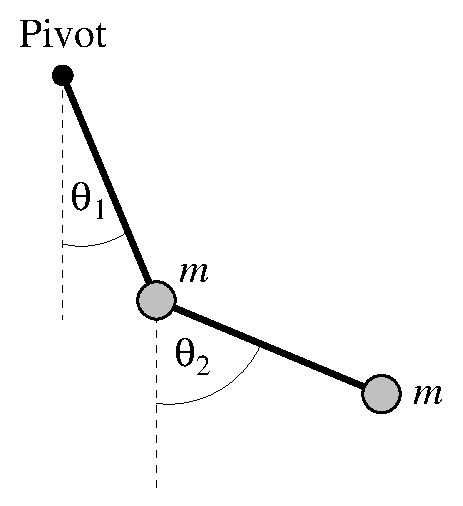
\includegraphics[width=4.5cm]{double.eps}
\end{center}

\noindent The position of the arms at any moment in time is uniquely
specified by the two angles $\theta_1$ and~$\theta_2$.  The
equations of motion for the angles are most easily derived using the
Lagrangian formalism, as follows.

The heights of the two bobs, measured from the level of the pivot are
\begin{displaymath}
h_1 = -\ell\cos\theta_1, \qquad
h_2 = -\ell(\cos\theta_1+\cos\theta_2),
\end{displaymath}
so the potential energy of the system is
\begin{displaymath}
V = mgh_1 + mgh_2 = -mg\ell(2\cos\theta_1 + \cos\theta_2),
\end{displaymath}
where $g$ is the acceleration due to gravity.
The (linear) velocities of the two bobs are given by
\begin{displaymath}
v_1 = \ell\dot\theta_1, \qquad
v_2^2 = \ell^2 \bigl[ \dot\theta_1^2 + \dot\theta_2^2
  + 2 \dot\theta_1\dot\theta_2 \cos(\theta_1-\theta_2) \bigr],
\end{displaymath}
where $\dot\theta$ means the derivative of $\theta$ with respect to
time~$t$.  (If you don't see where the second velocity equation comes from,
it's a good exercise to derive it for yourself from the geometry of the
pendulum.)  Now the total kinetic energy is
\begin{displaymath}
T = \half m v_1^2 + \half m v_2^2
  = m\ell^2 \bigl[ \dot\theta_1^2 + \half \dot\theta_2^2
  + \dot\theta_1\dot\theta_2 \cos(\theta_1-\theta_2) \bigr],
\end{displaymath}
and the Lagrangian of the system is
\begin{displaymath}
\mathcal{L} = T - V
  = m\ell^2 \bigl[ \dot\theta_1^2 + \half \dot\theta_2^2
  + \dot\theta_1\dot\theta_2 \cos(\theta_1-\theta_2) \bigr]
  + mg\ell(2\cos\theta_1 + \cos\theta_2).
\end{displaymath}
Then the equations of motion are given by the Euler--Lagrange equations
\begin{displaymath}
{\dd\over\dd t} \biggl({\partial\mathcal{L}\over\partial\dot\theta_1} \biggr)
  = {\partial\mathcal{L}\over\partial\theta_1}, \qquad
{\dd\over\dd t} \biggl({\partial\mathcal{L}\over\partial\dot\theta_2} \biggr)
  = {\partial\mathcal{L}\over\partial\theta_2},
\end{displaymath}
which in this case give
\begin{align*}
2\ddot\theta_1 + \ddot\theta_2 \cos(\theta_1-\theta_2)
  &+ \dot\theta_2^2 \sin(\theta_1-\theta_2) + 2{g\over\ell} \sin\theta_1 = 0,
  \\
\ddot\theta_2 + \ddot\theta_1 \cos(\theta_1-\theta_2)
  &- \dot\theta_1^2 \sin(\theta_1-\theta_2) + {g\over\ell} \sin\theta_2 = 0,
\end{align*}
where the mass~$m$ has canceled out.

These are second-order equations, but we can convert them into first-order
ones by the usual method, defining two new variables,
$\omega_1$~and~$\omega_2$, thus:
\begin{displaymath}
\dot\theta_1 = \omega_1,\qquad \dot\theta_2 = \omega_2.
\end{displaymath}
In terms of these variables our equations of motion become
\begin{align*}
2\dot\omega_1 + \dot\omega_2 \cos(\theta_1-\theta_2)
  &+ \omega_2^2 \sin(\theta_1-\theta_2) + 2{g\over\ell} \sin\theta_1 = 0,
  \\
\dot\omega_2 + \dot\omega_1 \cos(\theta_1-\theta_2)
  &- \omega_1^2 \sin(\theta_1-\theta_2) + {g\over\ell} \sin\theta_2 = 0.
\end{align*}
Finally we have to rearrange these into the standard form of Eq.~(8.29)
with a single derivative on the left-hand side of each one, which gives
\begin{align*}
\dot\omega_1 &= - {\omega_1^2\sin(2\theta_1-2\theta_2)
                + 2\omega_2^2\sin(\theta_1-\theta_2)
                + (g/\ell) \bigl[ \sin(\theta_1-2\theta_2)
                                  + 3 \sin\theta_1 \bigr]\over
                 3 - \cos(2\theta_1-2\theta_2)}, \\
\dot\omega_2 &= {4\omega_1^2\sin(\theta_1-\theta_2)
                + \omega_2^2\sin(2\theta_1-2\theta_2)
                + 2(g/\ell) \bigl[ \sin(2\theta_1-\theta_2)
                                   - \sin\theta_2 \bigr]\over
                3 - \cos(2\theta_1-2\theta_2)}.
\end{align*}
(This last step is quite tricky and involves some trigonometric identities.
If you're not certain of how the calculation goes you may find it useful to
go through the derivation for yourself.)

These two equations, along with the equations $\dot{\theta}_1=\omega_1$ and
$\dot{\theta}_2=\omega_2$, give us four first-order equations which between
them define the motion of the double pendulum.
\begin{enumerate}\setlength{\itemsep}{0pt}
\item Derive an expression for the total energy $E = T + V$ of the system
  in terms of the variables $\theta_1$, $\theta_2$, $\omega_1$,
  and~$\omega_2$, plus the constants $g$, $\ell$, and~$m$.
\item Write a program using the fourth-order Runge--Kutta method to solve
  the equations of motion for the case where $\ell=40\,$cm, with the
  initial conditions $\theta_1=\theta_2=90^\circ$ and
  $\omega_1=\omega_2=0$.  Use your program to calculate the total energy of
  the system assuming that the mass of the bobs is $1\,$kg each, and make a
  graph of energy as a function of time from $t=0$ to $t=100$ seconds.

  Because of energy conservation, the total energy should be constant over
  time (actually it should be zero for this particular set of initial
  conditions), but you will find that it is not perfectly constant because
  of the approximate nature of the solution of the differential equation.
  Choose a suitable value of the step size~$h$ to ensure that the variation
  in energy is less than~$10^{-5}$~Joules over the course of the
  calculation.

\item Make a copy of your program and modify the copy to create a second
  program that does not produce a graph, but instead makes an animation of
  the motion of the double pendulum over time.  At a minimum, the animation
  should show the two arms and the two bobs.

  Hint: As in Exercise~8.4 you will probably find the function \verb|rate|
  useful in order to make your program run at a steady speed.  You will
  probably also find that the value of~$h$ needed to get the required
  accuracy in your solution gives a frame-rate much faster than any that
  can reasonably be displayed in your animation, so you won't be able to
  display every time-step of the calculation in the animation.  Instead you
  will have to arrange the program so that it updates the animation only
  once every several Runge--Kutta steps.
\end{enumerate}


%%% Exercise 8.16 %%%

\exercise \textbf{The three-body problem}

\exskip If you mastered Exercise~8.10 on cometary orbits, here's a more
challenging problem in celestial mechanics---and a classic in the
field---the \defn{three-body problem}.

  Three stars, in otherwise empty space, are initially at rest, with the
  following masses and positions, in arbitrary units:
\begin{center}
\begin{tabular}{l|crr}
       & Mass & $x$ & $y$ \\
\hline
Star 1 & 150 & 3 & 1 \\
Star 2 & 200 & $-1$ & $-2$ \\
Star 3 & 250 & $-1$ & 1
\end{tabular}
\end{center}
(All the $z$ coordinates are zero, so the three stars lie in the $xy$
plane.)
\begin{enumerate}\setlength{\itemsep}{0pt}
\item Show that the equation of motion governing the position~$\vec{r}_1$
  of the first star is
\begin{displaymath}
{\dd^2\vec{r}_1\over\dd t^2}
  = Gm_2{\vec{r}_2-\vec{r}_1\over|\vec{r}_2-\vec{r}_1|^3}
    + Gm_3{\vec{r}_3-\vec{r}_1\over|\vec{r}_3-\vec{r}_1|^3}
\end{displaymath}
and derive two similar equations for the positions $\vec{r}_2$ and
$\vec{r}_3$ of the other two stars.  Then convert the three second-order
equations into six equivalent first-order equations, using the techniques
you have learned.
\item Working in units where $G=1$, write a program to solve your equations
  and hence calculate the motion of the stars from $t=0$ to $t=2$.  Make a
  plot showing the trails of all three stars (i.e.,~a graph of $y$
  against~$x$ for each star).
\item Modify your program to make an animation of the motion on the screen
  from $t=0$ to $t=10$.  You may wish to make the three stars different
  sizes or colors (or both) so that you can tell which is which.
\end{enumerate}
To do this calculation properly you will need to use an adaptive step size
method, for the same reasons as in Exercise~8.10---the stars move very
rapidly when they are close together and very slowly when they are far
apart.  An adaptive method is the only way to get the accuracy you need in
the fast-moving parts of the motion without wasting hours uselessly
calculating the slow parts with a tiny step size.  Construct your program
so that it introduces an error of no more than $10^{-3}$ in the position of
any star per unit time.

Creating an animation with an adaptive step size can be challenging,
since the steps do not all correspond to the same amount of real time.  The
simplest thing to do is just to ignore the varying step sizes and make an
animation as if they were all equal, updating the positions of the stars on
the screen at every step or every several steps.  This will give you a
reasonable visualization of the motion, but it will look a little odd
because the stars will slow down, rather than speed up, as they come close
together, because the adaptive calculation will automatically take more
steps in this region.

A better solution is to vary the frame-rate of your animation so that the
frames run proportionally faster when $h$ is smaller, meaning that the
frame-rate needs to be equal to $C/h$ for some constant~$C$.  You can
achieve this by using the \verb|rate| function from the
\verb|visual| package to set a different frame-rate on each step, equal to
$C/h$.  If you do this, it's a good idea to not let the value of~$h$ grow
too large, or the animation will make some large jumps that look uneven on
the screen.  Insert extra program lines to ensure that $h$ never exceeds a
value~$h_\textrm{max}$ that you choose.  Values for the constants of around
$C=0.1$ and $h_\textrm{max}=10^{-3}$ seem to give reasonable results.


%%% Exercise 8.17 %%%

\exercise \textbf{Cometary orbits and the Bulirsch--Stoer method}

\exskip Repeat the calculation of the cometary orbit in Exercise~8.10
(page~361) using the adaptive Bulirsch--Stoer method of Section~8.5.6 to
calculate a solution accurate to $\delta=1$~kilometer per year in the
position of the comet.  Calculate the solution from $t=0$ to
$t=2\times10^9\,$s, initially using just a single time interval of size
$H=2\times10^9\,$s and allowing a maximum of $n=8$ modified midpoint steps
before dividing the interval in half and trying again.  Then these
intervals may be subdivided again, as described in Section~8.5.6, as many
times as necessary until the method converges in eight steps or less in
each interval.

Make a plot of the orbit (i.e.,~a plot of $y$ against~$x$) and have your
program add dots to the trajectory to show where the ends of the time
intervals lie.  You should see the time intervals getting shorter in the
part of the trajectory close to the Sun, where the comet is moving rapidly.

Hint: The simplest way to do this calculation is to make use of recursion,
the ability of a Python function to call itself.  (If you're not familiar
with the idea of recursion you might like to look at Exercise~2.13 on
page~83 before doing this exercise.)  Write a user-defined function called,
say, \verb|step(r,t,H)| that takes as arguments the position vector
$\vec{r} = (x,y)$ at a starting time~$t$ and an interval length~$H$, and
returns the new value of $\vec{r}$ at time $t+H$.  This function should
perform the modified midpoint/Richardson extrapolation calculation
described in Section~8.5.5 until either the calculation converges to the
required accuracy or you reach the maximum number $n=8$ of modified
midpoint steps.  If it fails to converge in eight steps, have your function
call itself, twice, to calculate separately the solution for the first then
the second half of the interval from $t$ to $t+H$, something like this:
\begin{code}
r1 = step(r,t,H/2)
r2 = step(r1,t+H/2,H/2)
\end{code}
(Then \emph{these} functions can call themselves, and so forth, subdividing
the interval as many times as necessary to reach the required accuracy.)


%%% Exercise 8.18 %%%

\exercise \textbf{Oscillating chemical reactions}

\exskip The \defn{Belousov--Zhabotinsky reaction} is a chemical
oscillator, a cocktail of chemicals which, when heated, undergoes a series
of reactions that cause the chemical concentrations in the mixture to
oscillate between two extremes.  You can add an indicator dye to the
reaction which changes color depending on the concentrations and watch the
mixture switch back and forth between two different colors for as long as
you go on heating the mixture.

Physicist Ilya Prigogine formulated a mathematical model of this type of
chemical oscillator, which he called the ``Brusselator'' after his
home town of Brussels.  The equations for the Brusselator are
\begin{displaymath}
{\dd x\over\dd t} = 1 - (b+1)x + ax^2y, \qquad
{\dd y\over\dd t} = bx - ax^2y.
\end{displaymath}
Here $x$ and $y$ represent concentrations of chemicals and $a$ and $b$ are
positive constants.

Write a program to solve these equations for the case $a=1$, $b=3$ with
initial conditions $x=y=0$, to an accuracy of at least $\delta=10^{-10}$
per unit time in both $x$ and~$y$, using the adaptive Bulirsch--Stoer
method described in Section~8.5.6.  Calculate a solution from $t=0$ to
$t=20$, initially using a single time interval of size $H=20$.  Allow a
maximum of $n=8$ modified midpoint steps in an interval before you divide
in half and try again.

Make a plot of your solutions for $x$ and $y$ as a function of time, both
on the same graph, and have your program add dots to the curves to show
where the boundaries of the time intervals lie.  You should find that the
points are significantly closer together in parts of the solution where the
variables are changing rapidly.

Hint: The simplest way to perform the calculation is to make use of
recursion, as described in Exercise~8.17.

\end{exercises}

\end{document}
